\documentclass[10pt]{standalone}
\usepackage{amsmath}
\usepackage{amssymb}
\usepackage{pgf,tikz}
\usepackage{mathrsfs}
\usetikzlibrary{arrows}
\pagestyle{empty}

\begin{document}

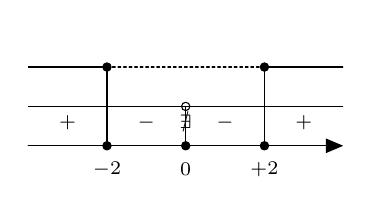
\begin{tikzpicture}[line cap=round,line join=round,>=triangle 45,x=1.0cm,y=1.0cm]

\draw[->,color=black] (-0.0,0.) -- (4.0,0.);


\clip(0.0,-0.5) rectangle (4.0,1.5);
\draw (0.,0.5)-- (4.,0.5);
\draw (2.,0.5)-- (2.,0.);
\draw (1.,1.)-- (1.,0.);
\draw (3.,1.)-- (3.,0.);
\draw (0.,1.)-- (1.,1.);
\draw [dash pattern=on 1pt off 1pt] (1.,1.)-- (3.,1.);
\draw (3.,1.)-- (4.,1.);
\begin{scriptsize}
\draw [fill=black] (2.,0.) circle (1.5pt);
\draw (2.0,-0.3) node {$0$};
\draw (2.0,0.3) node {$\nexists$};
\draw  (2.,0.5) circle (1.5pt);
\draw [fill=black] (1.,0.) circle (1.5pt);
\draw (1.0,-0.3) node {$-2$};
\draw [fill=black] (1.,1.) circle (1.5pt);
\draw [fill=black] (3.,0.) circle (1.5pt);
\draw (3.0,-0.3) node {$+2$};
\draw [fill=black] (3.,1.) circle (1.5pt);
\draw (0.5,+0.3) node {$+$};
\draw (1.5,+0.3) node {$-$};
\draw (2.5,+0.3) node {$-$};
\draw (3.5,+0.3) node {$+$};
\end{scriptsize}
\end{tikzpicture}
\end{document}